\documentclass{prose-report}
% \usepackage[utf8]{inputenc}
\usepackage[T1]{fontenc}
\usepackage{lipsum}
\usepackage{changepage}
\usepackage{graphicx}
\usepackage{float}
\usepackage{calc}
\usepackage[export]{adjustbox}
\usepackage{lettrine}
\usepackage[table]{xcolor}
\usepackage{colortbl}
\usepackage{roboto}

\arrayrulecolor{gray!50}

\dochead{TESS follow-up}
\title{TOI-2091.02}
\author{2020 10 10 $\cdot$ Artemis $\cdot$ I+z}
\date{}

%================

\begin{document}
{\fontfamily{cmss}\selectfont
\maketitle

% {
% \makebox[\paperwidth+1.8cm][r]{
%   \raisebox{-\totalheight + 6cm}[0pt][0pt]{
%     \includegraphics[angle=30, width=13cm]{tess}
%   }
%  }
% }

\begin{tabular}{m{0.3\linewidth}m{0.25\linewidth}m{0.2\linewidth}}
\parbox{\linewidth}{
  \boxtitle{NIGHT}
  \mbox{\hspace{-0.7cm}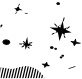
\includegraphics[width=\linewidth + 0.7cm]{figures/stars}}
  \vspace{-1cm}\newline

  {\bgroup
  \def\arraystretch{1.2}% 
  \tiny
  \rowcolors{1}{white}{gray!8}
  \roboto
  \begin{tabular}{|m{0.45\linewidth}|m{0.45\linewidth}|}
    \hline
     \textcolor{black!50}{Time} & 20:42 - 00:44 [4h2]\\
    \hline
     \textcolor{black!50}{RA - DEC} & 17 17 02.10 - +72 44 49.3\\
    \hline
     \textcolor{black!50}{images} & 484\\
    \hline
    \textcolor{black!50}{Some} & Some values\\
    \hline
    \textcolor{black!50}{mean std · fwhm} &  1.51 · 3.56 pixels \\
    \hline
    \textcolor{black!50}{exposure} & 20.0 s \\
  \hline
  \end{tabular}
  \egroup}

  \boxtitle{PSF}
  \mbox{\hspace{-0.92cm}\includegraphics[width=\linewidth + 0.92cm]{figures/psf}}
  {\bgroup
  \def\arraystretch{1.2}% 
  \tiny
  \rowcolors{1}{white}{gray!8}
  \roboto
  \begin{tabular}{|m{0.45\linewidth}|m{0.45\linewidth}|}
    \hline
     \textcolor{black!50}{Time} & 20:42 - 00:44 [4h2]\\
    \hline
     \textcolor{black!50}{RA - DEC} & 17 17 02.10 - +72 44 49.3\\
    \hline
     \textcolor{black!50}{images} & 484\\
    \hline
    \textcolor{black!50}{Some} & Some values\\
    \hline
    \textcolor{black!50}{mean std · fwhm} &  1.51 · 3.56 pixels \\
    \hline
    \textcolor{black!50}{exposure} & 20.0 s \\
  \hline
  \end{tabular}
  \egroup}
  \newline
} & \hspace{0.7cm}\parbox{\linewidth}{
  \boxtitle{LIGHTCURVE}
  \mbox{\hspace{-1cm}\includegraphics[width=\linewidth + 1cm]{figures/lightcurve}}
  {\centering{\footnotesize model: $f = c + fwhm^2 + sky^2 + T + \epsilon$}}

  \boxtitle{RAW}
  \mbox{\hspace{-0.8cm}\includegraphics[width=\linewidth + 0.8cm]{figures/raw}}
} & \hspace{1.5cm}\parbox{\linewidth}{
  
\boxtitle{SYSTEMATICS}
  \mbox{\hspace{-0.9cm}\includegraphics[width=\linewidth + 0.9cm]{figures/systematics}}\\
  
  \boxtitle{COMPARISON STARS}
  \mbox{\hspace{-0.9cm}\includegraphics[width=\linewidth + 0.9cm]{figures/comparison}}
} \\
\end{tabular}


$$
\left(\!
    \begin{array}{c}
      n \\
      r
    \end{array}
  \!\right) = \frac{n!}{r!(n-r)!}
$$


  \lipsum[5]
  \lipsum[66]
  \lipsum[66]
  \lipsum[66]
  \lipsum[1-10]
  \lipsum[66]
}
\end{document}